\documentclass[12pt,a4paper]{article}
\usepackage{graphicx}
\usepackage{url}

\begin{document}

\begin{titlepage}

\center{\Huge{The Black Box}}
\center{\large{Perception in the 19th century}}
\vspace{1cm}

\begin{figure}[h]
	\centering
	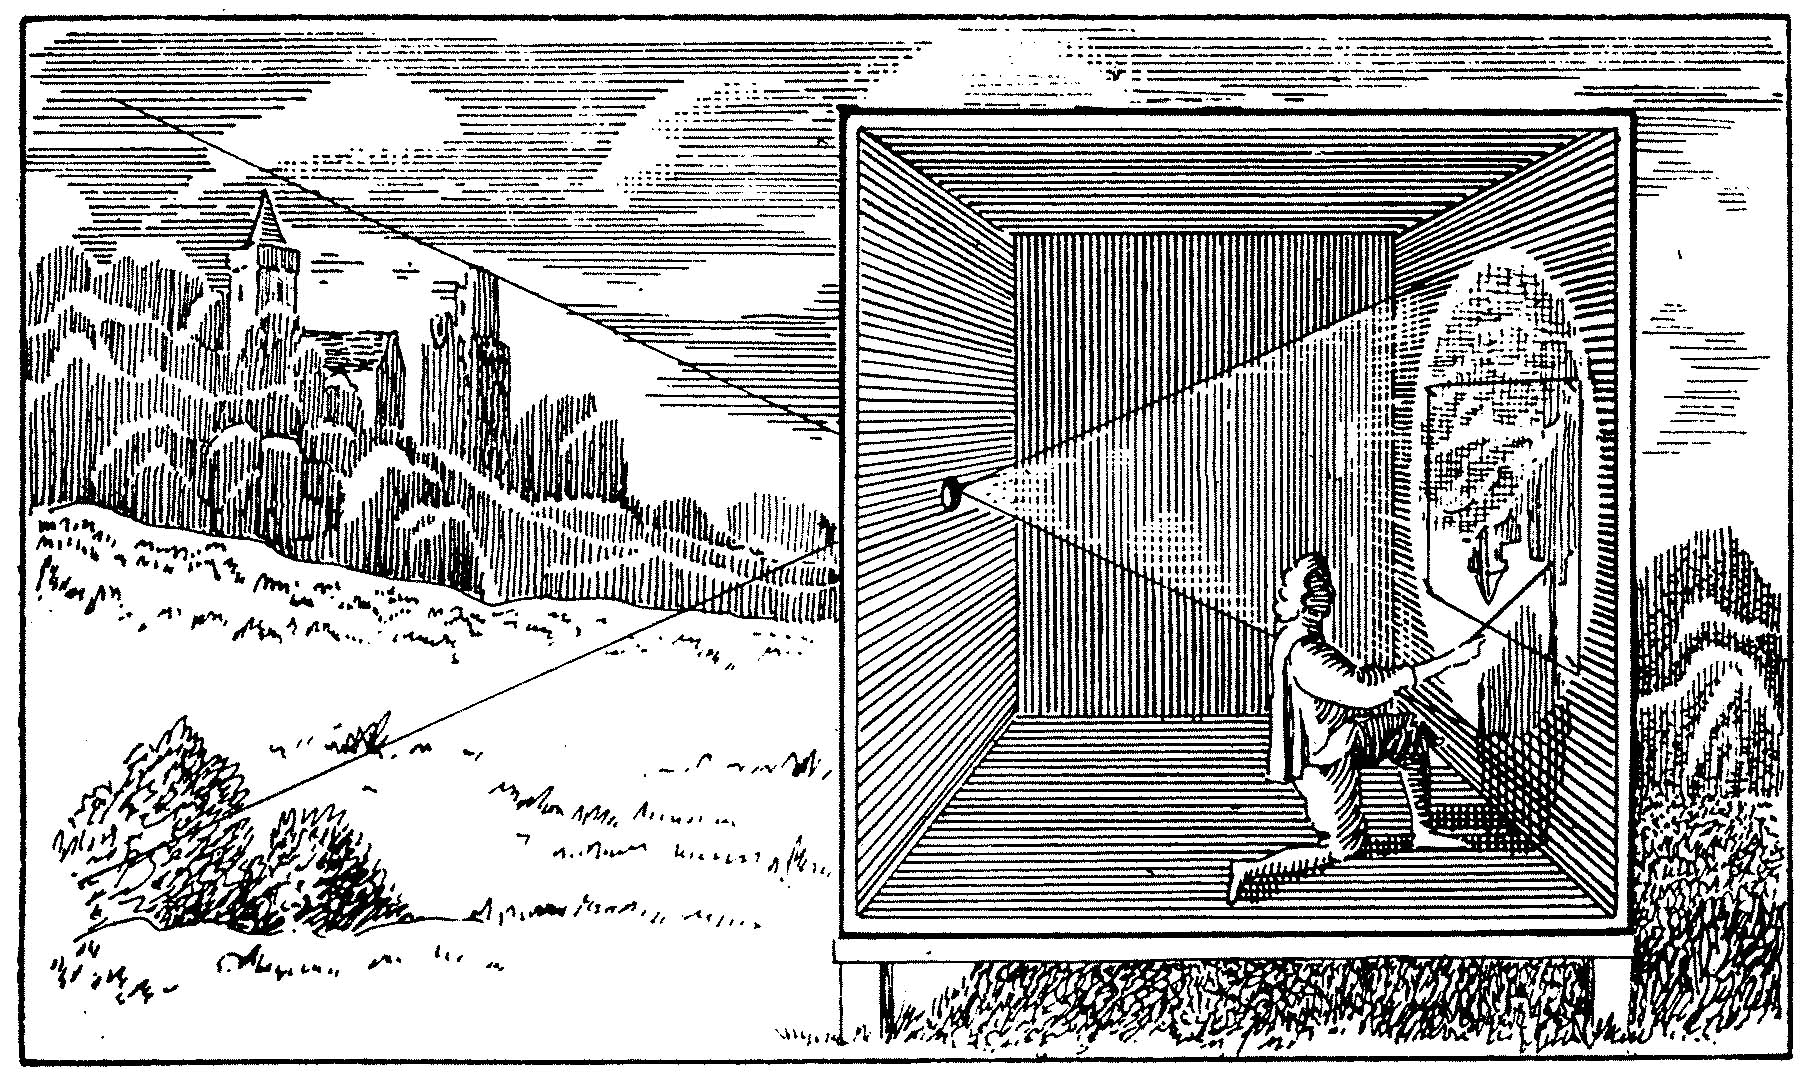
\includegraphics[width=\textwidth]{img/cameraobscura.jpeg}
\end{figure}

\vspace{1cm}
\center{Dominik Schlegel}
\center{\today}

\end{titlepage}


\newpage

\section*{Preface}

On the following pages I will discuss the development of the human perception model and its
inseparable relations to the scientific body in the 19th century. The essay focusses on
{\it{Subjective Vision and the Separation of the Senses}} \cite{crary} and includes information from
{\it{Techniques of the Observer}} \cite{crary}, {\it{The Images of Precision: Helmholtz and the
graphical Method in Physiology}} \cite{holmes} and {\it{Camera and Mind}} \cite{ellenbogen}. Basic
knowledge of the material is assumed and only the key points will be repeated in order to explain
my view.

As an additional, diverse source I picked a topic about the beginning of the institutionalization of people
with disabilities during the 19th century and its direct connection to the respective idea of
perception and human society \cite{earlymovement}.

\section*{Thesis}

I claim that the change from the 18th centuries humanly passive and pseudo-objective
perception to the physiologically objective perception of the 19th century was crucial in order to
enable the massive growth in production of scientific knowledge during the 19th century.
The human body was far from being completely understood at the end of the 18th century but
nevertheless people took perceived impressions as the undiluted, completely clear representation of
their true nature.
This premise reduces the observer to a simple, passive receiver of information without any transformation
of the input from outside - which is not entirely true as we know nowadays.
One can easily think about the numerous possible conflicts resulting from parties with differently developed
senses (e.g. eyesight).

At the same time researches started to play around with the senses and challenged this humanly passive model
of perception. As a result people became unsure about the intake of their senses and the human body
manifested itself as the nature of perception (from physics to physiology). The human body can therefore be
seen as a black box, an object in which we do not not what is going on but in which we expect a
transformation of the input. The step to the acceptance of this black box is of prime importance to me.
Having the black box model researchers could start to quantify perception and get closer to truth
representations of nature.

Additionally one should not forget the inherent link between the new model of perception and human society.
The researchers pursuing this model of perception had many contestants and had a hard time publishing
their findings in the beginning of the physiological movement.

Relating to my second source, people whose senses were non- or malfunctional were not able to perceive nature
based on the humanly passive model - and as a consequence were not accepted by the broad human society. This
changed with the model of perception, whereas it became clear that every human transforms nature and
therefore nobody can tell the actual truth of an occurrence. I do not say that this was the major reason for
rise of the institutionalization of people with disabilities but it certainly did play its part.

\section*{Reading}

{\it{Subjective Vision and the Separation of the Senses}} is a chapter of the book {\it{Techniques of the
Observer}} \cite{crary} written by Jonathan Crary. The essay is composed upon a literature collection and
refers to various famous historical figures. The two major topics discussed are the rise of physiology and
the establishment and reframing of new sciences.

In the following sections I will cover the main aspects of the reading and relate them to my Thesis.
Since the topics sometimes overlap with sections discussed in other readings, I will include that
information and mention the respective sources.

\subsection*{Camera Obscura and Subjective Vision}

The camera obscura is an optical device based on the principle of the pinhole camera model \cite{camera}. While
the principle has been known to mankind since approximately 400 BCE, a sufficiently precise realization of the
camera obscura was not achieved until the end of the 16th century. In the 17th century more people began to
work with the device and some started to develop theories about its relation to the human observer.

One of them was Isaac Newton who showed that a ray of white light - the portion of light passing through the
inlet of the camera obscura could be separated into the rainbow colors by using a prism \cite{newtongoethe}.
Newton published his findings in his major work: {\it{Opticks or a treatise of the reflections, refractions,
inflections andcolours of light}} \cite{opticks}.
It is important to note that the influence of physiology on perception
was not part of Newton's studies. The camera obscura established unclouded relations between
the artificial world inside the box and the natural world outside and enabled a clear separation
and definition of object and observer. The observer himself was not of interest for Newton and therefore the
possible correctness of observations was not challenged nor verified in terms of quality.

Over a hundred years later Johann Wolfgang von Goethe made the camera obscura the site of his optical studies
as well. Goethe summarises his work in {\it{'Farbenlehre'}} \cite{farbenlehre}. 
Goethe denied and battled Newton's theories about white light. For Goethe white light was the visible
absence of color whereas for Newton white light was the sum of all colors - this is a crucial difference
with correspondingly diverse resulting theories. As we know by today Newton was right, but at that time it
was not clear which theory is correct and Goethe made important discoveries, even though he seemed to be on
the wrong path from the start.

In contrast to Newton, Goethe started to involve physiology in his optical studies. This is the point where
the question of the human black box will turn up. Goethe created the perfect scenario for displaying the
physiological effects on the sense of sight and therefore on the observer by only a minimal modification of the
camera obscura: Goethe sealed the hole after a short aperture time.

The observer could now still experience an image even thought there was no
light source present. This contradicts the logic behind an observer seeing only real objects visible to him.
The resulting shift from a constant, passive, objective observer to a physiologically active, subjective
observer defines the human body as the active producer of an optical experience and as a direct
consequence, of all sensory experiences.
Thanks to this step the existence of a black box, the human perception as an active system became
undeniable. One speciality about Goethe's observer model is the inseparability of two models usually
presented as distinct and contradictory: the observer as a strictly physiological system and the
autonomous, independent producer of his/her own experiences.

At the same time other researchers such as Immanuel Kant strengthen this change of the point of view
in vision with their discoveries. William Blakes agrees on the model and Michel Foucault
emphasizes the the inconsistent relation to the old model.

Goethe and other researchers continued working with the sense of sight and began to discover
properties of the black box.
This means that the human itself started to examine the complex properties of its perception
in form of a legion of researchers for the first time. Because of the complexity of this topic
straight and efficient progress is not expected and researchers had numerous conflicts with
their colleagues in certain fields. Even though the conflicts slowed down the derivation of a
universal model, they guaranteed the maximum variety of studies to select from.

Later on Arthur Schopenhauer came up with heavily physiological theories on the subject. Schopenhauer
abandoned the combination of the two models Goethe used for his observer. According to Schopenhauer
the experience of color could only result from physiological phenomena. Even thought they disagreed on
that specific topic, both of them were against the Newtonian optics. Schopenhauer also rejected any model
of the observer as passive receiver of sensation as described by John Locke and Étienne Bonnot de Condillac.
The notion of correspondence between subject and object disappears for Schopenhauer and he
builds the complete perceptional apparatus upon the body of the observer. For him the distinction of
interior and exterior is irrelevant since it is only a construction of the human mind.

Starting from a simple optical device, the camera obscura and intense involvement in the sense of sight
Schopenhauer ended up questioning the view of reality. Schopenhauer also contested the works of Kant
and defined 'Vorstellung' as pure physiological phenomenon and criticizes the pure philosophical nature
of Kant's work. Another figure which was of grate importance to Schopenhauer was Xavier Bichat.
He provided Schopenhauer with a crucial physical model of the human subject helping him to manifest
his theories and had the same strong physiological ideologies as Schopenhauer.

The author preserves a neutral stance over the complete section and is able to provide
very dense information in a enjoyable way. The important background knowledge about occurring
personalities is not reserved and the reader can get a deep insight into the respective events.
The focus lies primarily on Goethe and as the text advances on Schopenhauer which gives an important spice
to the covered topics. Whereas I am only concerned about the main points regarding the evolution of the
model of perception the author lists various specific developments in great detail and mentions their
influence on the subject.

I end this section with a quote from the author which, in my opinion could not have better caught
the essence of the topic:

\begin{quote}

The subjective vision affirmed by Goethe and Schopenhauer that endowed the observer with a new perceptual
autonomy also coincided with the making of the observer into a subject of new knowledge and new
techniques of power. The terrain on which these two interrelated observers emerged in the nineteenth
century was the science of physiology. 

{\it{Subjective Vision and the Separation of the Senses}} \cite{crary}, page 79 first paragraph

\end{quote}

\subsection*{The Rise of Physiology}

Keeping the quote from the previous section in mind we move on to the discussion of the
emerge of physiology as a science.
It is clear that the strongly increasing occurrence of physiological aspects in the studies of many
prestigious researches demanded a institutionalization of physiology. Even thought the involvement
of physiology began already before the 19th century it became not formally specialized before 1940.
This change signalled how the human body was becoming the center of power and truth.
Scientists explored the aspects of the human body in great depth and by 1826, Johannes Müller
determined that sensory nerves are of five types. A first quantification of the black box has been made.
At the same time Pierre Flourens was able to identify functions of the different parts of the human
brain. A discretization of the brain into cerebellum, motor center and cerebrum, a perception center,
was the result his studies.

The ongoing evolution of physiology provided Schopenhauer with sufficient amounts of information to
ground his theories and vice versa. He isolated the perceptional part from the human body and
focussed on the way how reality is created by the observer. It became clear that perception is not
uniform in all men or women and therefore the black box can not be generalized. Schopenhauers urge to
find the pure objectivity of perception was extraordinary. Another important point is that
Schopenhauer insisted on the possibility of physical methods manipulating the certain modes of
perception. Relating to his remarkable physiological description of beauty one can easily see that
a cup of water is more appealing to a thirsty hiker just returning from the desert than to a
guy swimming in a mountain spring. It is assumed that both persons appreciate a cup of water to
the same amount if they are located in the same physical environment.
The cup of water is in the same physical condition in both cases but the observer underlies different
conditions, the perception is modified by physical stimuli.

The study of the eye was also an important part of another growing new discipline: the science of
physiological psychology. Here the relation to economy becomes visible, by a quantification of
perception processes could be optimized and executed more efficiently. One example would be just the
coordination of eye and hand which is required in almost every profession. The resulting
knowledge enabled techniques for the external control of the observer, the physical methods
Schopenhauer was already aware of.

By 1821 the wave theory of light had its major breakthrough thanks to Augustin Jean Fresnel.
This change made many of the large classical theories in optics obsolete.

\newpage

\subsection*{Techniques of the Observer}

\subsection*{The Graphical Method}

\subsection*{Camera and Mind}


\newpage

\bibliographystyle{unsrt}
\bibliography{references.bib}

\end{document}
